\section{Introducción}

\subsection{Circuito de Chua}

\begin{frame}
	\frametitle{\subsecname}

	\begin{itemize}
		\item

		      El \alert{circuito de Chua} es un sistema de ecuaciones diferenciales
		      ordinarias autónomo no lineal.

		\item

		      Para la realización de este circuito se añadió la restricción de que
		      el circuito tenga una \alert{resistencia no lineal} $N_{R}$ de dos
		      terminales de naturaleza lineal a trozos.

		\item

		      En el presente trabajo estudiaremos el comportamiento caótico del
		      circuito y el \alert{método de convergencia de órbitas} que nos
		      ayudará a estabilizar el mismo.
	\end{itemize}

	\begin{minipage}{0.45\textwidth}
		\begin{align*}
			\diff{V_{C_{1}}}{t} & =\frac{1}{RC_{1}}(V_{C_{2}} - V_{C_{1}} - g(V_{C_{1}})) \\
			\diff{V_{C_{2}}}{t} & =\frac{1}{RC_{2}}(V_{C_{1}} - V_{C_{2}} + Ri_{L})       \\
			\diff{i_{L}}{t}     & =-\frac{1}{L}V_{C_{2}}
		\end{align*}
		donde $V_{C_{1}}$, $V_{C_{2}}$ son los voltajes en los capacitores $C_{1}$, $C_{2}$,
		$R$ es la resistencia lineal,
		$L$ es la inductancia lineal, $i_{L}$ es la intensidad de corriente.
	\end{minipage}
	\begin{minipage}{0.45\textwidth}
		\begin{figure}[ht!]
			\centering
			\includesvg[width=0.35\paperwidth]{chua_circuit}
			\caption{Un circuito de Chua.}\label{fig:chua_circuit}
		\end{figure}
	\end{minipage}

\end{frame}
\note{
	El término diodo de Chua es una descripción general de una resistencia no lineal de dos terminales
	con curva característica lineal por tramos.

	El diode de Chua no es único.
}

\subsection{Ecuación de Chua adimensional}

\begin{frame}
	\frametitle{\subsecname}
	% Vea la figura~\ref{fig:chua_circuit}.

	\begin{minipage}{0.45\textwidth}
		\begin{align*}
			\diff{x}{t} & = \alpha\left(y - x - g\left(x\right)\right) \\
			\diff{y}{t} & = x - y + z                                  \\
			\diff{z}{t} & = -\beta y
		\end{align*}
		donde
		\begin{equation*}
			g\left(x\right)=
			\begin{cases}
				m_{0}x + m_{0} + m_{1} & \text{si } x\leq -1,   \\
				m_{1}x                 & \text{si } -1 < x < 1, \\
				m_{0}x + m_{1} - m_{0} & \text{si } x \geq 1.
			\end{cases}
		\end{equation*}
		y cuyos puntos de equilibrio son
		\begin{align*}
			P^{+} & =\left(1,0,-1\right) \\
			O     & =\left(0,0,0\right)  \\
			P^{-} & =\left(-1,0,1\right) \\
		\end{align*}
	\end{minipage}
	\begin{minipage}{0.45\textwidth}
		\begin{figure}[ht!]
			\centering
			\includesvg[width=0.35\paperwidth]{characteristic_curve}
			\caption{Curva caracterísitica de la resistencia no lineal $g\left(x\right)$.}\label{fig:piecewise}%Intensidad de corriente versus voltaje.
		\end{figure}
	\end{minipage}
\end{frame}
\note{
	Es antisimétrica, osea $\left(x,y,z\right)\to\left(-x,-y,z\right)$ no cambia la ecuación.
}

\subsection{Mapa de Poincaré}

\begin{frame}
	\frametitle{\subsecname}

	\begin{minipage}{0.6\textwidth}
		\begin{definition}{Mapa de Poincaré}{poincaremap}
			Es la aplicación que asocia los puntos en $V\subset\Sigma$ abierto
			tal que las trayectorias que inician en $V$ retornan a $\Sigma$
			\begin{align*}
				P\colon V & \to\Sigma                                      \\
				x         & \mapsto\phi\left(\tau\left(x\right), x\right),
			\end{align*}
			donde $\tau\left(x\right)$ es el primer retorno del punto $x$ a $\Sigma$.
			Además, decimos que $\Sigma$ es la sección transversal al campo vectorial
			$\diff{x}{t}=f\left(x\right)$, $x\left(t_{0}\right)=x_{0}$.
		\end{definition}
	\end{minipage}
	\begin{minipage}{0.3\textwidth}
		\begin{figure}[ht!]
			\centering
			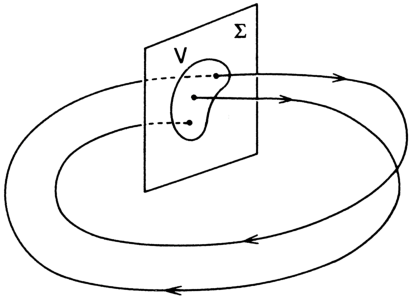
\includegraphics[width=0.35\paperwidth]{poincaremap}
			% \caption{Mapa de Poincaré para una órbita periódica.}\label{fig:poincaremap}
		\end{figure}
	\end{minipage}

\end{frame}

\note{
	$V\subset\Sigma$ abierto (por el teorema de existencia y unicidad para un campo vectorial $f$ de clase $C^{r}$)
}


\section{Método para determinar el caos}

\begin{frame}
	\frametitle{\secname}

	\begin{figure}[ht!]
		\centering
		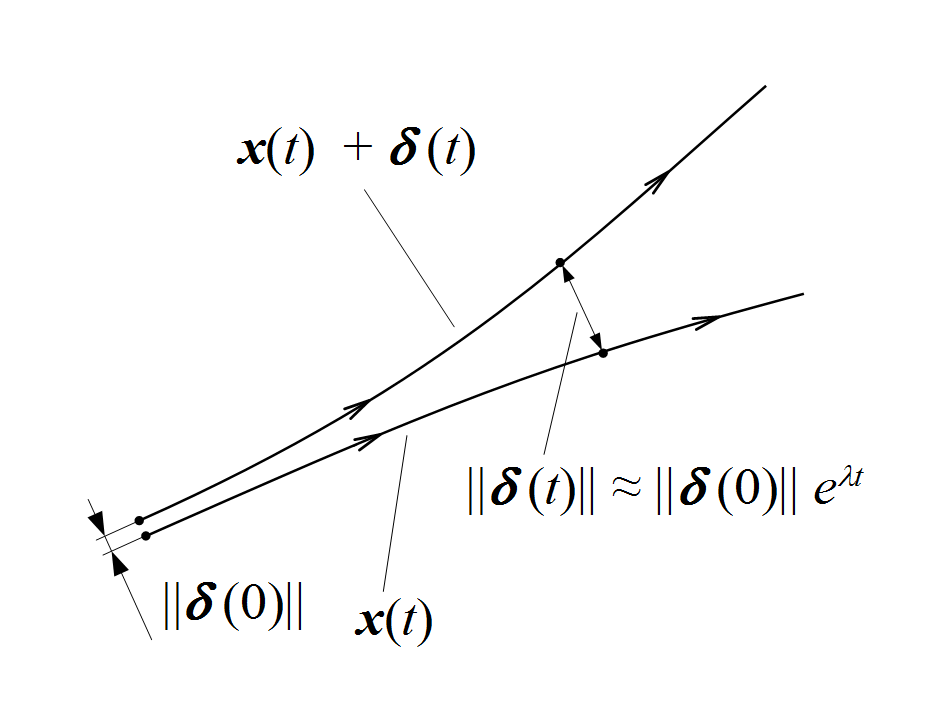
\includegraphics[width=0.7\paperwidth]{lyapunov}
		%\caption{}\label{fig:lyapunov}
	\end{figure}
\end{frame}

\section{Experimentos numéricos}

\begin{frame}
	\frametitle{\secname\quad$\left(\alpha=10.0, \beta=16.4, m_{0}=-1.22, m_{1}=0.628\right)$}

	\begin{minipage}{0.45\textwidth}
		\begin{figure}[ht!]
			\centering
			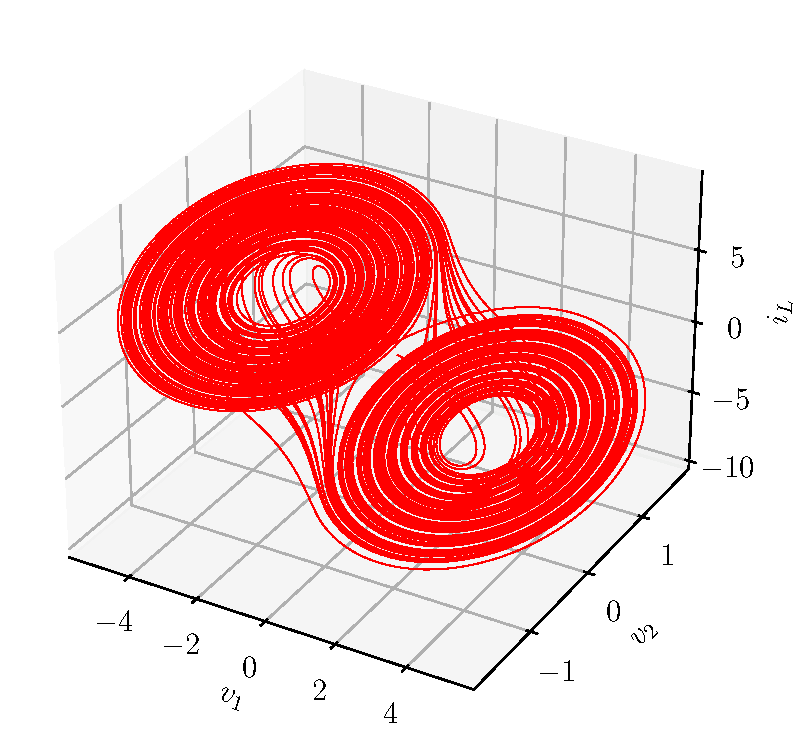
\includegraphics[width=0.45\paperwidth]{doble_atractor_chua}
			\caption{Sistema dinámico del doble atractor de Chua.}\label{fig:doble_atractor_chua}
		\end{figure}
	\end{minipage}
	\begin{minipage}{0.45\textwidth}
		\begin{figure}[ht!]
			\centering
			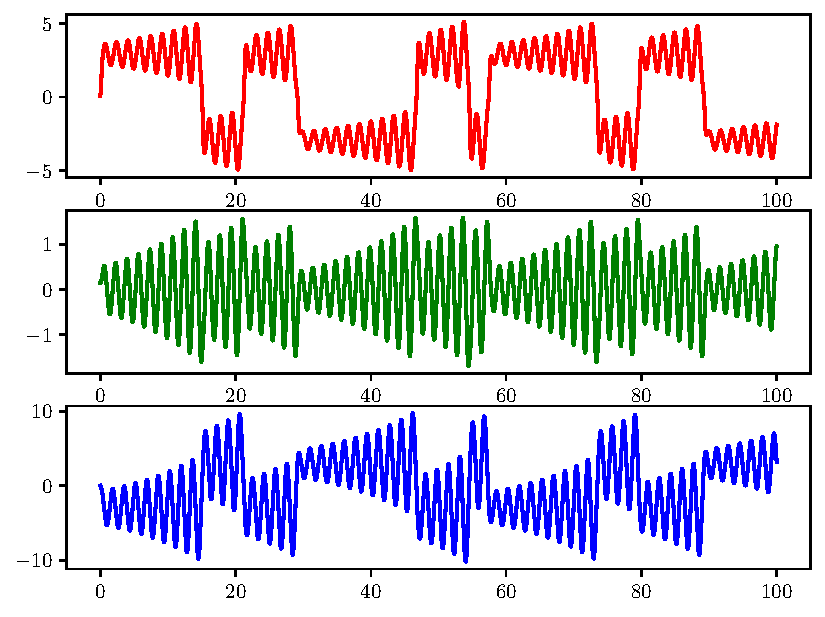
\includegraphics[width=0.45\paperwidth]{chua_solutions}
			\caption{Serie de tiempo.}\label{fig:chua_solutions}
		\end{figure}
	\end{minipage}
\end{frame}

\begin{frame}
	\frametitle{\secname\quad$\left(\beta_{1}=16.4,\beta_{2}=16.401\right)$}

	\begin{figure}[ht!]
		\centering
		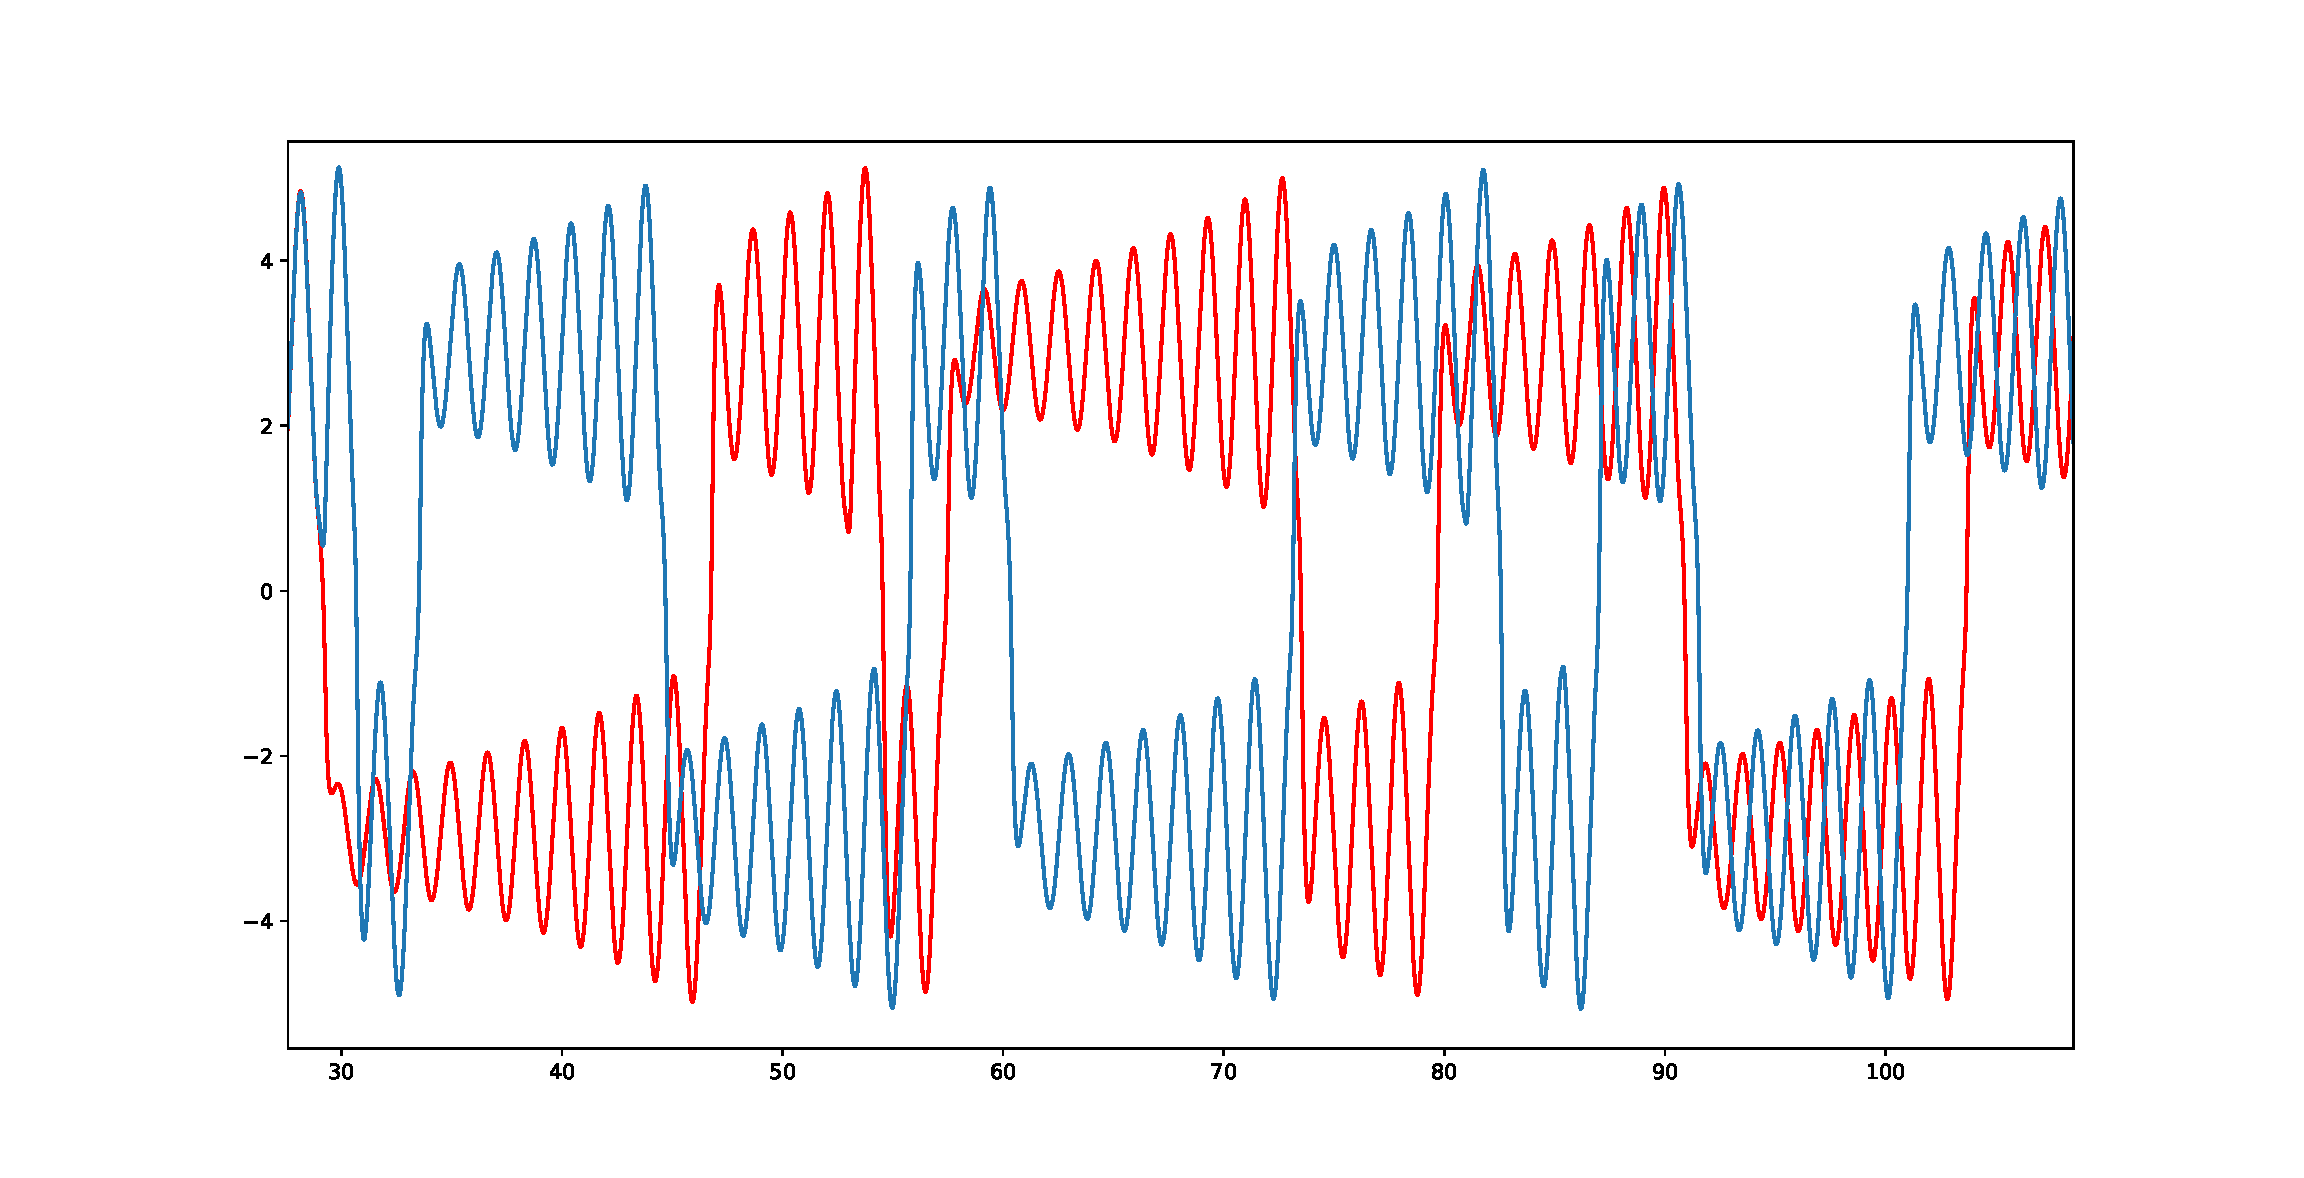
\includegraphics[width=0.9\paperwidth]{cambiando_el_beta}
		\caption{Azul: $\beta_{1}$, rojo: $\beta_{2}$.}\label{fig:lyapunov}
	\end{figure}

\end{frame}

\begin{frame}
	\frametitle{\secname\quad$\left(\alpha=10,\beta=16.4,R=-1.22,C_{2}=0.728\right)$}

	\begin{minipage}{0.45\textwidth}
		\begin{figure}[ht!]
			\centering
			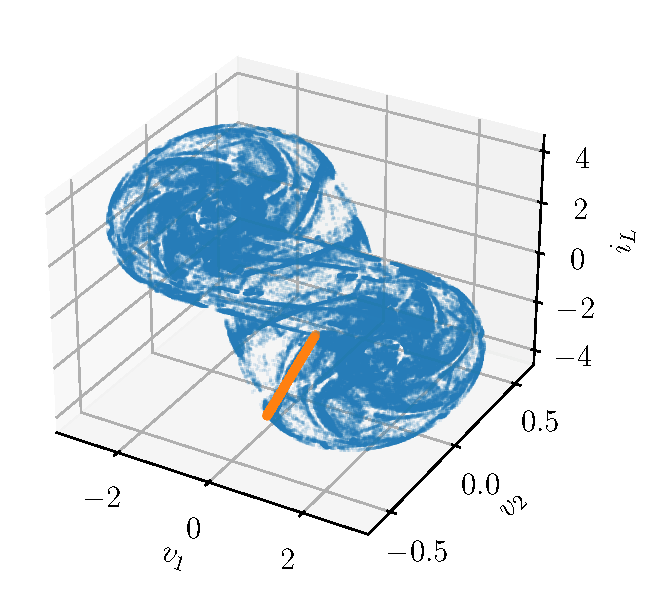
\includegraphics[width=0.44\paperwidth]{chua_doble_atractor}
			\caption{La sección transversal es el plano $x=1$ en el doble atractor de Chua.}\label{fig:chua_doble_atractor}
		\end{figure}
	\end{minipage}
	\begin{minipage}{0.45\textwidth}
		\begin{figure}[ht!]
			\centering
			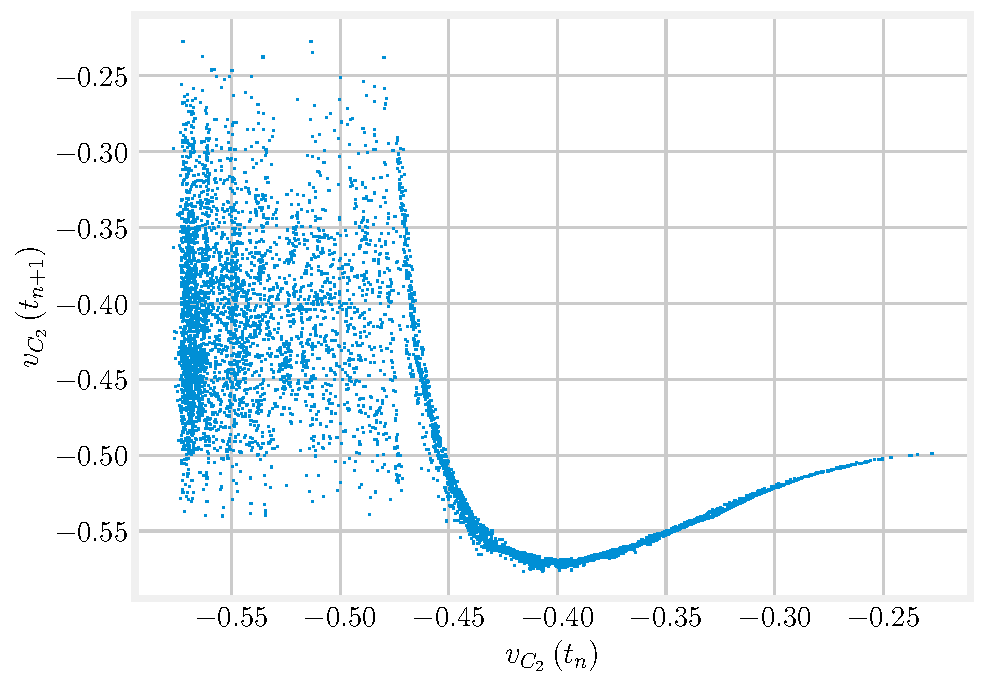
\includegraphics[width=0.44\paperwidth]{t_n_versus_y}
			\caption{Mapa de Poincaré: $y\left(t_{n}\right)$ versus $y\left(t_{n+1}\right)$.}\label{fig:chua_solutions}
		\end{figure}
	\end{minipage}
\end{frame}

\section{Programas}

\begin{frame}[fragile]
	\frametitle{\secname}
	\begin{minipage}{0.45\textwidth}
		Vea el Programa.
	\end{minipage}
	\begin{minipage}{0.45\textwidth}
		\inputminted[fontsize=\tiny, highlightlines={13-16,28-30,33-38}, firstline=1, lastline=41]{python}{poincare_chua.py}
	\end{minipage}
\end{frame}

\section{Conclusiones}

\begin{frame}
	\frametitle{\secname}
	\begin{itemize}
		\item De la figura podemos ver que el sistema de Chua bajo ciertos parámetros $\alpha= 10$  y $\beta_{1}=16.4$, $\beta_{2}=16.401$ es un sistemas caótico ya que para parámetros muy cercanos obtenemos soluciones muy diferentes.
		\item Para ciertos parámetros el sistema de Chua se comporta de manera caótica.
		\item De la figura logramos implementar un programa para poder obtener la sección de Poincaré y hacer las gráficas para hallar el mapa de primer retorno con el objetivo de ver si las órbitas sean estables. % Con la base de este programa podremos analizar otros sistemas caóticos. % Aplicaciones con la encriptación, redes neuronales.
	\end{itemize}
\end{frame}
